\documentclass{article}
\usepackage{graphicx}
% Include the minted package
\usepackage{minted}

\begin{document}
\section*{Simulation of the fractional coalescent with two populations}
The simulation code \texttt{simtree.py} will be available in our private GitHub [address need to be inserted].
Here, a few examples of the output are shown.
The key code is given in the snippet in Figure \ref{fig1}. Figure \ref{fig2} gives examples for two populations with different $\alpha$, all histograms were drawn from 5000 independent replicates using the same effective population sizes ($\Theta_1=0.01$,$\Theta_2=0.01$) and immigration rates ($M_{2\rightarrow1}=100$, $M_{1\rightarrow2}=100$), but different $\alpha$. Each histogram is compared with the standard Kingman coalescent.
\begin{figure}[h]
% Include your Python code
\begin{minted}{python}
# generates Mittag-Leffler time interval based on mylambda and alpha
# for each evolutionary force: Theta_1, Theta_2, M_21, M_12
# for the future, I assume this also will work for growth and population divergence 
# with the correct lambda 
def randommlftime(mylambda, alpha):
    pia = 3.1415926 * alpha
    r1 = np.random.uniform(0,1)
    r2 = np.random.uniform(0,1)
    denoma = 1.0 / alpha
    denomlambda = 1.0 / mylambda
    return -denomlambda**denoma * 
         (np.sin(pia)/(np.tan(pia*(1.0-r1)))-np.cos(pia))**denoma * 
         np.log(r2)

# creates the time for a migration or coalescent event,
# evaluating the time intervals for each force and picks the smallest
# looping through Y , the alphas vector here needs and entry for every force
# see the function fill_Yalphas()                                                                                                 
def randomtime(Y,alphas,t0):
    smallu = 1e100
    for yi,ai in zip(Y,alphas):
        u = randommlftime(yi,ai)
        if u < smallu:
            smallu = u
    return t0 + smallu
\end{minted}
\caption{Key python function to draw new event times using the fractional coalescent with different $\alpha$ per population.}\label{fig1}
\end{figure}

\begin{figure}[h]
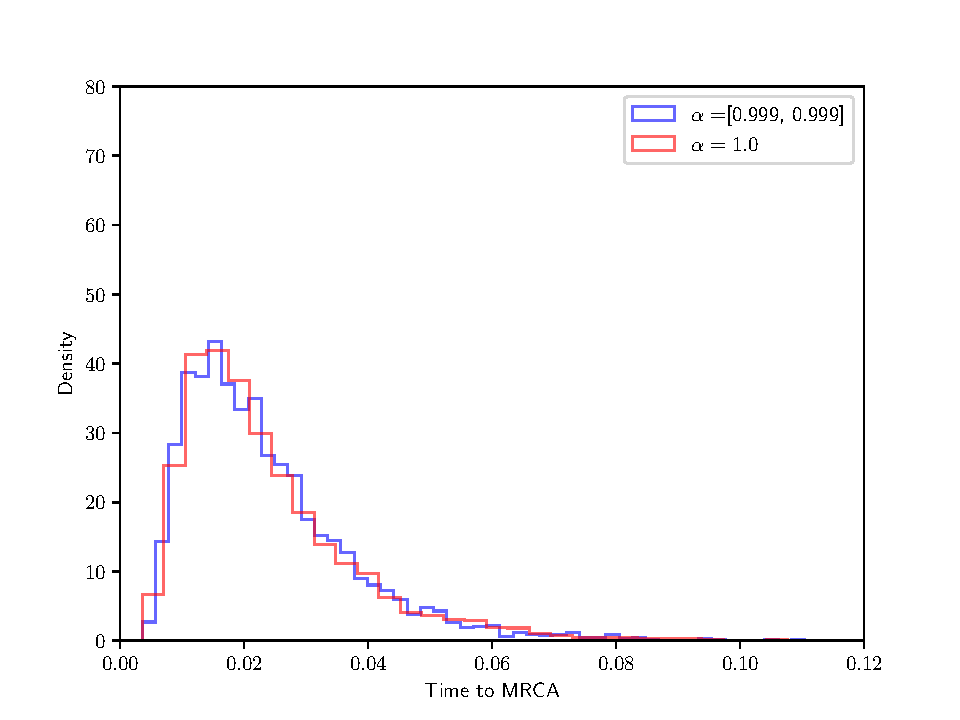
\includegraphics[width=0.32\textwidth]{simtree-0.999-0.999}
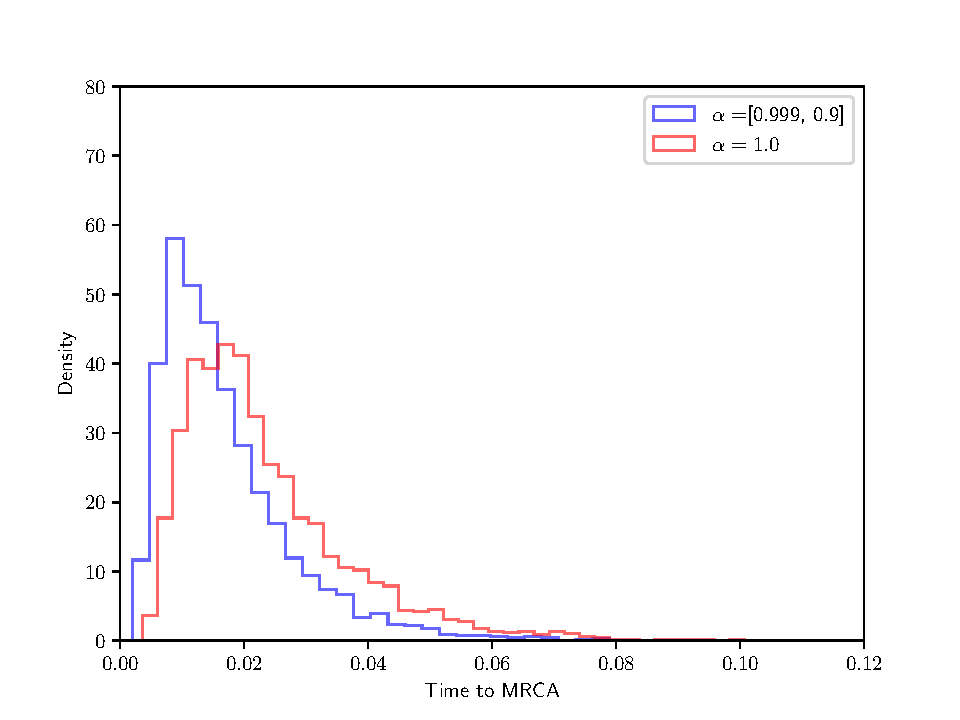
\includegraphics[width=0.32\textwidth]{simtree-0.999-0.9}
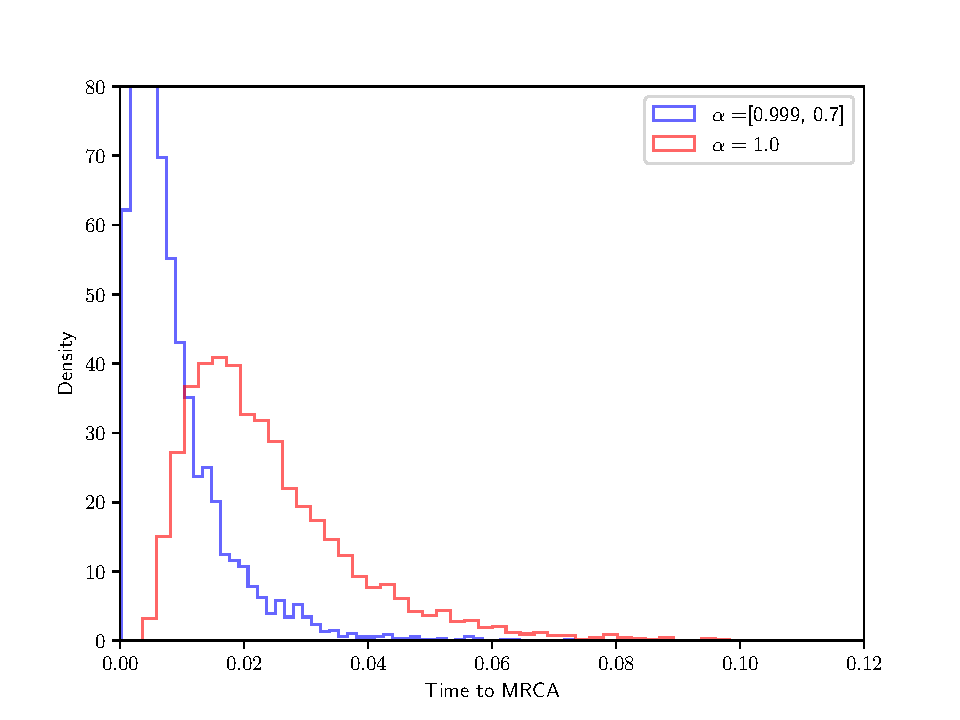
\includegraphics[width=0.32\textwidth]{simtree-0.999-0.7}\\
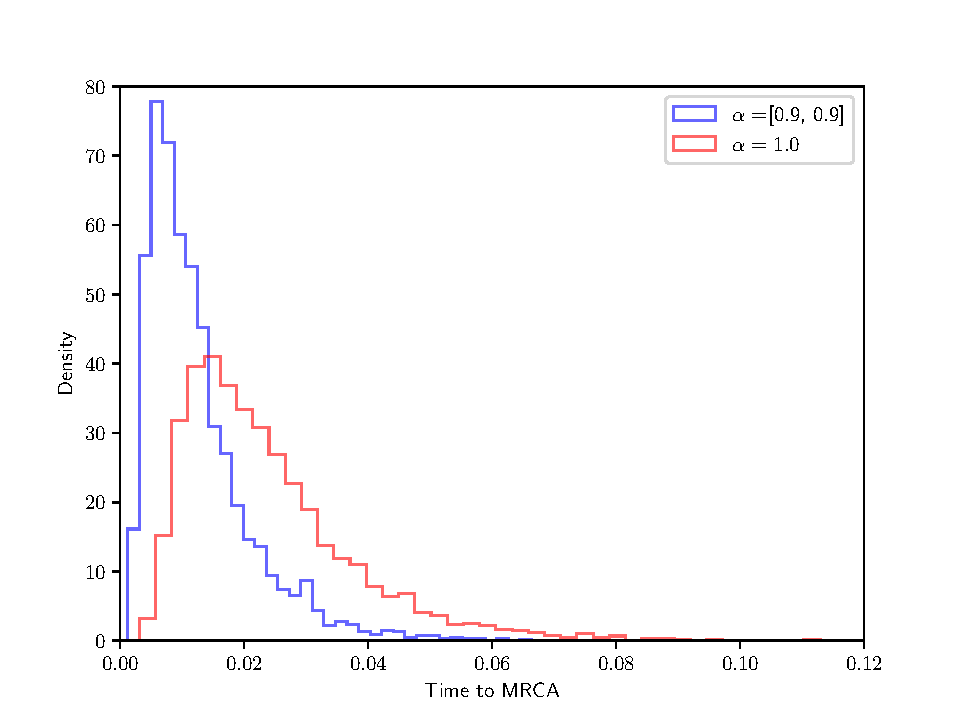
\includegraphics[width=0.32\textwidth]{simtree-0.9-0.9}
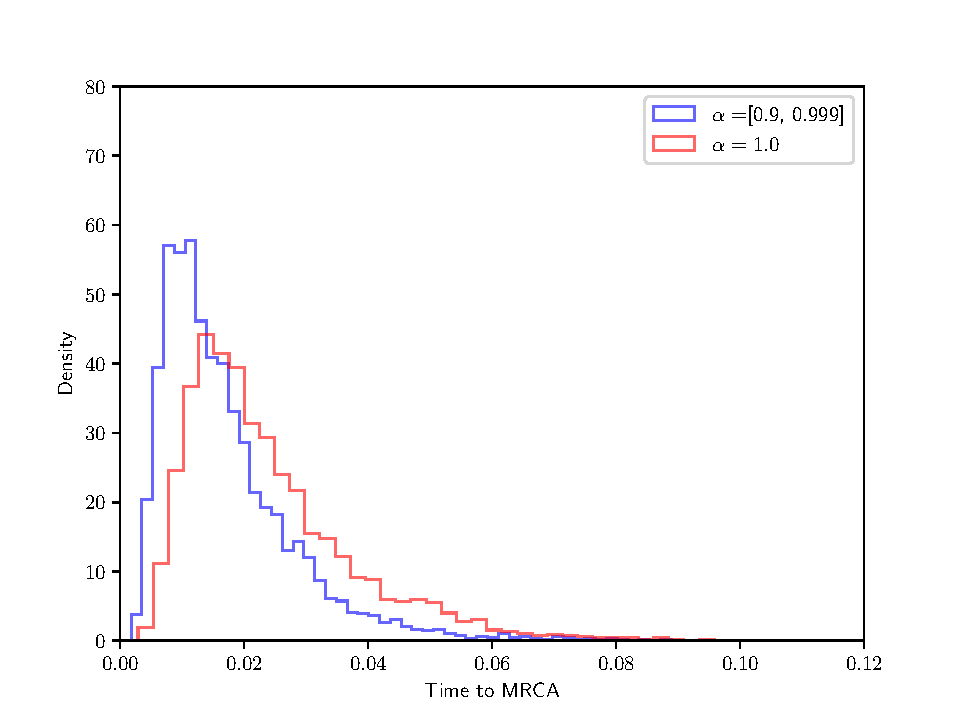
\includegraphics[width=0.32\textwidth]{simtree-0.9-0.999}
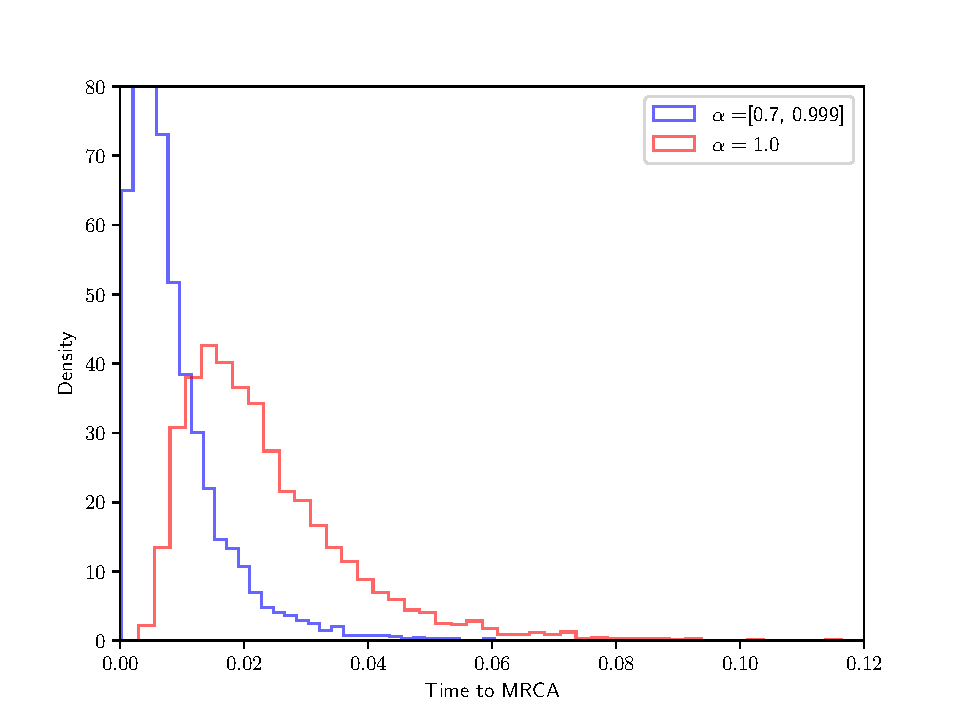
\includegraphics[width=0.32\textwidth]{simtree-0.7-0.999}
\caption{Comparison of six different scenarios for two populations with different $\alpha$: top left: both populations are essentially following the Kingman coalescent; top middle and right: one population deviates from the Kingman coalescent; bottom left: both populations deviate similarly from Kingman coalescent, bottom middle and right: Same scenario as `top middle and right' except that the $\alpha$ are reversed.}\label{fig2}
\end{figure}

\begin{samepage}

The script has several options:
\begin{verbatim}
usage: simtree.py [-h] [-l LOCI] 
                                    [-s SITES] 
                                    [-i INDIVIDUALS] 
                                    [-t THETA]
                                     [-m MIG] 
                                     [-a ALPHA] 
                                     [-f FILE] 
                                     [-p]

Simulate a tree

optional arguments:
  -h, --help            show this help message and exit
  -l LOCI, --loci LOCI  number of loci
  -s SITES, --sites SITES
                        number of sites
  -i INDIVIDUALS, --individuals INDIVIDUALS
                        Number of samples for each population
  -t THETA, --theta THETA
                        thetas for each population
  -m MIG, --mig MIG     migration rate for each population
  -a ALPHA, --alpha ALPHA
                        alpha for each population
  -f FILE, --file FILE  treefile to be used with migdata, default is NONE 
                                            which is a placeholder for sys.stdout
  -p, --plot            Plots density histogram of TMRCA
\end{verbatim}

\end{samepage}
\end{document}
